\documentclass[11pt]{article}
\usepackage{../cs70, latexsym,epsf,amsmath,amsfonts,graphicx,url,textcomp}
\lecture{16}
\def\title{Note \the\lecturenumber}

%%% Alistair's Macros
\makeatletter
\def\eqalign#1{\,\vcenter{\openup\jot\m@th
  \ialign{\strut\hfil${##}$&${{}##}$\hfil
      \crcr#1\crcr}}\,}
\def\eqalignno#1{\displ@y \tabskip\@centering
  \halign to\displaywidth{\hfil${##}$\tabskip\z@skip
    &${{}##}$\hfil\tabskip\@centering
    &\llap{$##$}\tabskip\z@skip\crcr
    #1\crcr}}
\makeatother
\def\third{{\textstyle{1\over 3}}}
\def\half{{\textstyle{1\over 2}}}
\def\quarter{{\textstyle{1\over 4}}}
\def\ul#1{\underline{#1}}
\def\Omega{\mathchar"10A }
\def\Omega{\mathchar"10A }
\newenvironment{proposition}{\par\global\advance\theoremnumber by 1
{\bf Proposition \the\lecturenumber.\the\theoremnumber}:
\begingroup\em}%
{\endgroup}
\def\ignore#1{}
\def\Ex#1{{\rm E}(#1)}
\def\Aset{{\cal A}}
%%% End Alistair's Macros

\newcounter{thm}
\addtocounter{thm}{\the\lecturenumber}
\newtheorem{theorem}{Theorem}[thm]
\newtheorem{definition}{Definition}[thm]

\begin{document}
\maketitle

\section*{Random Variables: Distribution and Expectation}

{\bf Example: Coin Flips}

\smallskip

Recall our setup of a probabilistic experiment as a procedure of drawing a sample from
a set of possible values, and assigning a probability for each possible outcome of the experiment.
For example, if we toss a fair coin $n$ times, then there are $2^n$ possible outcomes, each of which
is equally likely and has probability $\frac{1}{2^n}$.

Now suppose we want to make a measurement in our experiment. For example, we can ask
what is the number of heads in $n$ coin tosses; call this number $X$. Of course, $X$ is not a fixed number,
but it depends on the actual sequence of coin flips that we obtain. For example, if $n = 4$ and
we observe the outcome $\omega = HTHH$, then the number of heads is $X = 3$; whereas if we
observe the outcome $\omega = HTHT$, then the number of heads is $X = 2$. In this example of $n$ coin tosses
we only know that $X$ is an integer between $0$ and $n$, but we do not know what its exact value is
until we observe which outcome of $n$ coin flips is realized and count how many heads there are. Because
every possible outcome is assigned a probability, the value $X$ also carries with it a probability for each possible
value it can take. The table below lists all the possible values $X$ can take in the example of $n = 4$ coin tosses,
along with their respective probabilities.

\begin{center}\begin{tabular}{|c|c|c|}
\hline
outcomes $\omega$ & value of $X$ (number of heads) & probability occurring \\ \hline
TTTT & 0 & $1/16$ \\
HTTT, \:THTT, \:TTHT, \:TTTH & 1 & $4/16$ \\
HHTT, \,HTHT, \,HTTH, \,THHT, \,THTH, \,TTHH & 2 & $6/16$ \\
HHHT, \:HHTH, \:HTHH, \:THHH & 3 & $4/16$ \\
HHHH & 4 & $1/16$ \\ \hline
\end{tabular}\end{center}




Such a value $X$ that depends on the outcome of the probabilistic experiment is called
a {\em random variable} (or {\em r.v.}). As we see from the example above, $X$ does not have a definitive value, but
instead only has a probability {\em distribution} over the set of possible values $X$ can take, which is why
it is called random. So the question ``What is the number of heads in $n$ coin tosses?'' does not exactly
make sense because the answer $X$ is a random variable. But the question
``What is the {\em typical} number of heads in $n$ coin tosses?'' makes sense: it is asking what is the 
average value of $X$ (the number of heads) if we repeat the experiment of tossing $n$ coins
multiple times. This average value is called the {\em expectation} of $X$, and is one of the most useful summary
(also called {\em statistics}) of an experiment.
 
\smallskip

{\bf Example: Permutations}

\smallskip

Before we formalize all these notions, let us consider another example to enforce our
conceptual understanding of a random variable. Suppose we collect the homeworks
of $n$ students, randomly shuffle them, and return them to the students. How many students
receive their own homework?

Here the probability space consists of all $n!$ permutations of the homeworks,
each with equal probability $\frac{1}{n!}$. If we label the homeworks as $1,2,\dots,n$,
then each sample point is a permutation $\pi = (\pi_1,\dots,\pi_n)$ where $\pi_i$ is
the homework that is returned to the $i$-th student. Note that $\pi_1,\dots,\pi_n \in \{1,2,\dots,n\}$
are all distinct, so each element in $\{1,\dots,n\}$ appears exactly once in the permutation $\pi$.

In this setting, the $i$-th student receives her own homework if and only if $\pi_i = i$. Then the
question ``How many students receive their own homework?'' translates into the question
of how many indices $i$'s satisfy $\pi_i = i$. These are known as \ul{fixed points} of the permutation.
As in the coin flipping case above, our question does not have a simple numerical answer
(such as~4), because the number depends on the particular permutation we choose (i.e., on the sample point).
Let's call the number of fixed points~$X$, which is a random variable.

To illustrate the idea concretely, let's consider the example $n = 3$. The following
table gives a complete listing of the sample space (of size $3!=6$),
together with the corresponding value of~$X$ for each sample point. Here we see that
$X$ takes on values 0, 1 or~3, depending on the sample point.
You should check that you agree with this table.
\begin{center}\begin{tabular}{|c|c|}
\hline
permutation~$\pi$&value of $X$ (number of fixed points) \\\hline
123&3\\
132&1\\
213&1\\
231&0\\
312&0\\
321&1\\\hline
\end{tabular}\end{center}





\subsection*{Random Variables}
Let us formalize the concepts discussed above.

\begin{definition}[Random Variable]
A \ul{random variable}~$X$ on a sample space~$\Omega$ is a function
$X \colon \Omega \to \mathbb{R}$ that assigns to each sample point $\omega\in\Omega$
a real number~$X(\omega)$.
\end{definition}

Until further notice, we will restrict out attention to random variables
that are \ul{discrete}, i.e., they take values in a range that is finite
or countably infinite. This means even though we define $X$ to map $\Omega$ to $\mathbb{R}$,
the actual set of values $\{X(\omega) \colon \omega \in \Omega\}$ that $X$ takes is a discrete subset of $\mathbb{R}$.



A random variable can be visualized in general by the picture in Figure \ref{fig:rv}.\footnote{The figures in this note are inspired by figures in Chapter 2 of "Introduction to Probability" by D.~Bertsekas and J.~Tsitsiklis.} Note that the term ``random variable'' is really something of a misnomer: it is a function so there is nothing random about it and it is definitely not a variable! What is random is which sample point of the experiment is realized and hence the value that the random variable maps the sample point to.
 
\begin{figure}[h!t!b!p!]
\centering
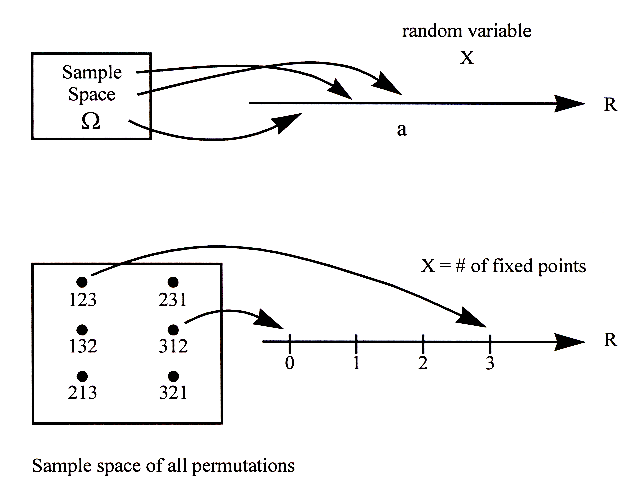
\includegraphics[scale=0.92]{rv}
\caption{Visualization of how a random variable is defined on the sample space.}
\label{fig:rv}
\end{figure}

\subsection*{Distribution}

When we introduced the basic probability space in Note~13, we defined two things:
\begin{enumerate} %\itemsep1pt
  \item the sample space $\Omega$ consisting of all the possible outcomes (sample points) of the experiment;
  \item the probability of each of the sample points.
\end{enumerate}

\pagebreak
Analogously, there are two things important about any random variable:
\begin{enumerate} %\itemsep1pt
  \item the set of values that it can take;
  \item the probabilities with which it takes on the values.
\end{enumerate}
Since a random variable is defined on a probability space, we can calculate these probabilities given the probabilities of the sample points.
Let $a$ be any number in  the range of a random variable~$X$.
Then the set $$
   \{\omega\in\Omega:X(\omega)=a\}  $$
is an {\it event\/} in the sample space (simply because it is a subset of $\Omega$).  We usually abbreviate
this event to simply ``$X=a$''.  Since $X=a$ is an event, we can
talk about its probability, $\Pr[X=a]$.  The collection of these
probabilities, for all possible values of~$a$, is known as the
{\it distribution\/} of the random variable~$X$.
\begin{definition}[Distribution]
The \ul{distribution} of a discrete random variable~$X$ is the
collection of values $\{(a,\Pr[X=a]):a\in\Aset\}$, where $\Aset$
is the set of all possible values taken by~$X$.
\end{definition}

Thus, the distribution of the random variable~$X$ in our permutation
example above is:
$$\Pr[X=0]={1\over 3};\qquad\Pr[X=1]={1\over 2};\qquad\Pr[X=3]={1\over 6}; $$
and $\Pr[X=a]=0$ for all other values of~$a$.

The distribution of a random variable can be visualized as a  bar diagram,  shown in Figure~\ref{fig:dist}. The $x$-axis represents the values that the random variable can take on. The  height of the bar at a value $a$ is the probability $\Pr[X=a]$. Each of these probabilities can be computed by looking at the probability of the corresponding event in the sample space.

\begin{figure}[h!]
\centering
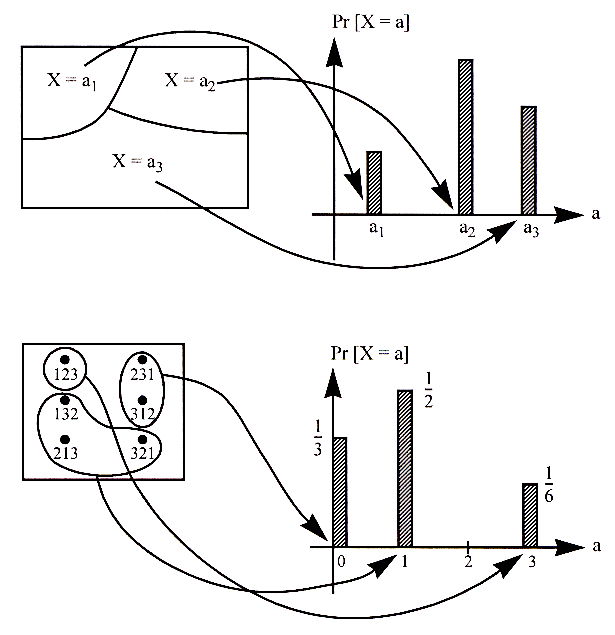
\includegraphics{distribution}
\caption{Visualization of how the distribution of a random variable is defined.}
\label{fig:dist}
\end{figure}


\pagebreak
Note that the collection of events $X=a$, $a \in \Aset$,  satisfy two important properties:
\begin{itemize}
\item Any two events $X=a_1$ and $X= a_2$ with $a_1 \not = a_2$ are disjoint.
\item The union of all these events is equal to the entire sample space $\Omega$.
\end{itemize}

The collection of events thus form a {\it partition} of the sample space (see Figure \ref{fig:dist}).  Both properties follow directly from the fact that $X$ is a function defined on $\Omega$, i.e., $X$ assigns a unique value to each and every possible sample point in $\Omega$.
As a consequence, the sum of the probabilities $\Pr[X=a]$ over all possible
values of~$a$ is exactly~1. So when we sum up the
probabilities of the events $X=a$, we are really summing up the
probabilities of all the sample points.


\subsubsection*{Example: The Binomial Distribution}
Let's return to our coin tossing example above, where we defined our random variable $X$ to be the number of heads. More formally, consider the random experiment consisting of $n$ independent tosses of a biased coin which lands on heads with probability $p$. Each sample point $\omega$ is a sequence of tosses. $X(\omega)$ is defined to be the number of heads in $\omega$. For example, when $n = 3$, $X(THH) = 2$. 

To compute the distribution  of $X$, we first enumerate the possible values $X$ can take on. They are simply $0, 1, \ldots, n$. Then we compute the probability of each event $X=i$ for $i =0, 1, \ldots, n$. The probability of the event $X=i$ is the sum of the probabilities of all the sample points with exactly $i$ heads (for example, if $n=3$ and $i=2$, there would be three such sample points $\{HHT, HTH, THH\}$). Any such sample point has a probability $p^i(1-p)^{n-i}$, since the coin flips are independent. There are exactly $n \choose i$ of these sample points. So
\begin{equation}
\Pr[X=i] = {n \choose i} p^i(1-p)^{n-i} \qquad \text{ for } ~ i =0,1, \ldots, n.
\end{equation}

This distribution, called the {\it binomial\/} distribution, is one of the most important distributions in probability. 
A random variable with this distribution is called a {\it binomial\/} random variable, written as
$$X \sim Bin(n,p)$$
An example of a binomial distribution is shown in Figure~\ref{fig:binomial}. Notice that due  to the properties of $X$ mentioned above, it must be the case that $\sum_{i=0}^{n}\Pr[X=i] = 1$, which implies that
$\sum_{i=0}^{n}{n \choose i}p^i(1-p)^{n-i} = 1$.  This provides a probabilistic proof
of the Binomial Theorem!

\begin{figure}[h!]
\centering
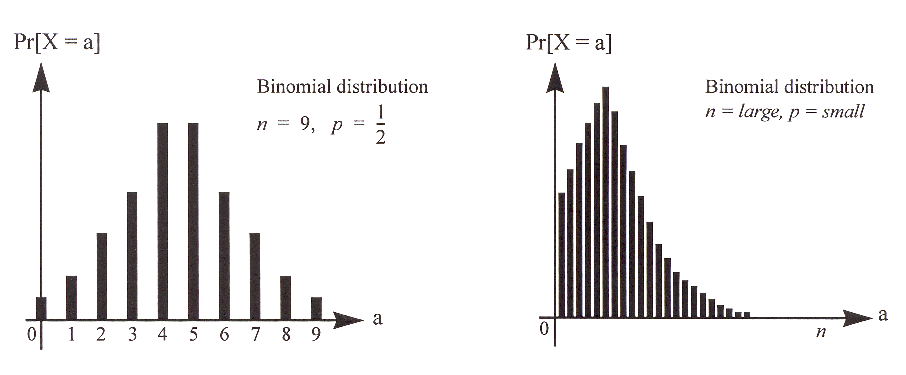
\includegraphics{binomial}
\caption{The binomial distributions for two choices of $(n,p)$.}
\label{fig:binomial}
\end{figure}

Although we define the binomial distribution in terms of an experiment involving tossing coins, this distribution is useful for modeling many real-world problems. Consider for example the error correction problem studied in Note~9. Recall that we wanted to encode $n$ packets into $n+k$ packets such that the recipient can reconstruct the original $n$ packets from any $n$ packets received. But in practice, the number of packet losses is random, so how do we choose $k$, the amount of redundancy? If we model each packet getting lost with probability $p$ and the losses are independent, then if we transmit $n+k$ packets, the number of packets received is a random variable $X$ with binomial distribution: $X \sim Bin(n+k,1-p)$ (we are tossing a coin $n+k$ times, and each coin turns out to be a head (packet received) with probability $1-p$).  So the probability
of successfully decoding the original data is:
$$ \Pr[X \ge n] ~=~ \sum_{i=n}^{n+k} \Pr[X = i] ~=~ \sum_{i=n}^{n+k} {n+k \choose i} (1-p)^i p^{n+k-i}.$$
Given fixed $n$ and $p$, we can choose $k$ such that this probability is no less than, say, $0.99$.



\subsection*{Expectation}

The distribution of a r.v.\ contains {\em all} the probabilistic information about the r.v.
In most applications, however, the complete distribution of a r.v.\ is
very hard to calculate. For example, consider the homework permutation example with $n = 20$. 
In principle, we'd have to enumerate $20!\approx 2.4\times10^{18}$ sample points, compute
the value of~$X$ at each one, and count the number of points
at which $X$ takes on each of its possible values! (though in
practice we could streamline this calculation a bit).
Moreover, even when we can compute the complete distribution
of a r.v., it is often not very informative.

For these reasons, we seek to {\it compress\/} the distribution into
a more compact, convenient form that is also easier to compute.
The most widely used such form is the {\it expectation\/}
(or {\it mean\/} or {\it average\/}) of the r.v.
\begin{definition}[Expectation]\label{Def:Expectation}
The \ul{expectation} of a discrete random variable~$X$ is
defined as $$
   \Ex{X}=\sum_{a\in\Aset} a\times\Pr[X=a], $$
where the sum is over all possible values taken by the r.v.
\end{definition}

For our simpler permutation example with only 3 students, the expectation is $$
   \Ex{X}=\left( 0\times{1\over 3}\right) +
          \left( 1\times{1\over 2}\right) +
          \left( 3\times{1\over 6}\right) =
          0+{1\over 2}+{1\over 2} = 1.  $$
That is, the expected number of fixed points in a permutation of three
items is exactly~1.

The expectation can be seen in some sense as a ``typical'' value
of the r.v.\ (though note that it may not actually be a value
that the r.v.\ ever takes on).  The question of how typical the
expectation is for a given r.v.\ is a very important one that we
shall return to in a later lecture.

Here is a physical interpretation of the expectation of a random variable:
imagine carving out a wooden cutout figure of the probability distribution
as in Figure~\ref{fig:gravity}. Then the expected value of the distribution is the balance point
(directly below the center of gravity) of this object. 

\begin{figure}[h!]
\centering
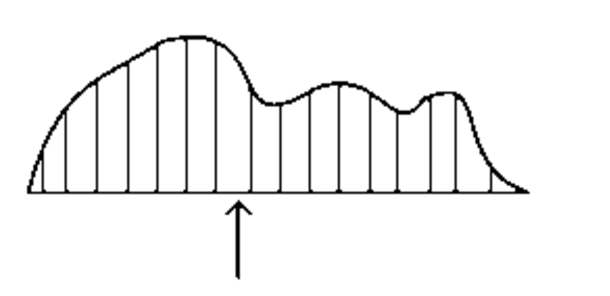
\includegraphics[scale=0.6]{gravity.pdf}
\caption{Physical interpretation of expected value as the balance point.}
\label{fig:gravity}
\end{figure}



\subsubsection*{Examples}
\begin{enumerate}

\item {\bf Single die.}  Throw one fair die.  Let $X$ be the
number that comes up.  Then $X$ takes on values $1,2,\ldots,6$
each with probability~$1\over 6$, so $$
   \Ex{X}={1\over 6}(1+2+3+4+5+6)={{21}\over 6} = {7\over 2}.  $$
Note that $X$ never actually takes on its expected value~$7\over 2$.

\item {\bf Two dice.}  Throw two fair dice.  Let $X$ be the sum
of their scores.  Then the distribution of $X$ is
\begin{center}\begin{tabular}{|c|ccccccccccc|}
\hline
$a$&2&3&4&5&6&7&8&9&10&11&12\\\hline\\[-12pt]
$\Pr[X=a]$&${1\over{36}}$&${1\over{18}}$&$1\over{12}$&$1\over 9$&$5\over{36}$&
           $1\over 6$&$5\over{36}$&$1\over 9$&$1\over{12}$&$1\over{18}$&$1\over{36}$\\[2pt]\hline
\end{tabular}\end{center}
The expectation is therefore $$
   \Ex{X}=\left(2\times{1\over{36}}\right)+\left(3\times{1\over{18}}\right)
          +\left(4\times{1\over{12}}\right)+\cdots+\left(12\times{1\over{36}}\right)=7.  $$

\item {\bf Roulette.}  A roulette wheel is spun (recall that a roulette wheel has 38
slots: the numbers $1,2,\ldots,36$, half of which are red and half black,
plus~0 and~00, which are green).  You bet \$1 on Black.
If a black number comes up, you receive your stake plus \$1; otherwise
you lose your stake.  Let $X$ be your net winnings in one game.  Then
$X$ can take on the values $+1$ and $-1$, and $\Pr[X=1]={{18}\over{38}}$,
$\Pr[X=-1]={{20}\over{38}}$.  Thus, $$
   \Ex{X} = \left(1\times{{18}\over{38}}\right) + \left(-1\times{{20}\over{38}}\right) = -{1\over{19}};  $$
i.e., you expect to lose about a nickel per game.
Notice how the zeros tip the balance in favor of the casino!
\end{enumerate}

\subsection*{Linearity of expectation}
So far, we've computed expectations by brute force: i.e., we have
written down the whole distribution and then added up the contributions
for all possible values of the r.v.  The real power of expectations
is that in many real-life examples they can be computed much more
easily using a simple shortcut.  The shortcut is the following:
\begin{theorem}\label{thmlin}
For any two random variables $X$ and~$Y$ on the same probability
space, we have $$
   \Ex{X+Y}=\Ex{X}+\Ex{Y}.  $$
Also, for any constant~$c$, we have $$
   \Ex{cX} = c\Ex{X}.  $$
\end{theorem}
\begin{proof}
To make the proof easier, we will first rewrite the definition of
expectation in a more convenient form.  Recall from Definition~\ref{Def:Expectation}
that $$
   \Ex{X}=\sum_{a\in\Aset} a\times\Pr[X=a].  $$
Let's look at one term $a\times\Pr[X=a]$ in the above sum.
Notice that $\Pr[X=a]$, by definition, is the sum of $\Pr[\omega]$
over those sample points~$\omega$ for which $X(\omega)=a$.
And we know that every sample point $\omega\in\Omega$ is in
exactly one of these events $X=a$.
This means we can write out the above definition in a more long-winded
form as
\begin{equation}\label{eqnewexp}
   \Ex{X}=\sum_{\omega\in\Omega} X(\omega)\times\Pr[\omega].
\end{equation}
This equivalent definition of expectation will make the present proof
much easier (though it is usually less convenient for actual calculations).

Now let's write out $\Ex{X+Y}$ using equation~(\ref{eqnewexp}):  $$
\eqalign{\Ex{X+Y}&=\sum_{\omega\in\Omega} (X+Y)(\omega)\times\Pr[\omega]\cr
                 &=\sum_{\omega\in\Omega} (X(\omega)+Y(\omega))\times\Pr[\omega]\cr
                 &=\sum_{\omega\in\Omega} \Bigl(X(\omega)\times\Pr[\omega]\Bigr) + \sum_{\omega\in\Omega} \Bigl(Y(\omega)\times\Pr[\omega]\Bigr)\cr
                 &= \Ex{X} + \Ex{Y}.\cr}  $$
In the last step, we used equation~(\ref{eqnewexp}) twice.

This completes the proof of the first equality.  The proof of
the second equality is much simpler and is left as an exercise.
\end{proof}

Theorem~\ref{thmlin} is very powerful: it says that the expectation
of a sum of r.v.'s is the sum of their expectations,
\ul{with no assumptions about the r.v.'s}. We
can use Theorem~\ref{thmlin} to conclude things like $\Ex{3X-5Y}=3\Ex{X}-5\Ex{Y}$.
This property is known as \ul{linearity of expectation}.

{\it Important caveat: Theorem~\ref{thmlin} does\/ {\bf not} say that
$\Ex{XY}=\Ex{X}\Ex{Y}$, or that $\Ex{{1\over X}}={1\over{\Ex{X}}}$,
etc.  These claims are not true in general.  It is only\/ {\rm sums}
and\/ {\rm differences} and\/ {\rm constant multiples} of random variables
that behave so nicely.}

\subsubsection*{Examples}
Now let's see some examples of Theorem~\ref{thmlin} in action.
\begin{enumerate}
\stepcounter{enumi}\stepcounter{enumi}\stepcounter{enumi}
\item {\bf Two dice again.}  Here's a much less painful way of computing
$\Ex{X}$, where $X$ is the sum of the scores of the two dice.  Note
that $X=X_1+X_2$, where $X_i$ is the score on die~$i$.  We know from
example~1 above that $\Ex{X_1}=\Ex{X_2}={7\over 2}$.  So by
Theorem~\ref{thmlin} we have $\Ex{X}=\Ex{X_1}+\Ex{X_2}=7$.
\item {\bf More roulette.}  Suppose we play the above roulette game
not once, but 1000 times.  Let $X$ be our expected net winnings.
Then $X=X_1+X_2+\ldots+X_{1000}$, where $X_i$ is our net winnings
in the $i$th play.  We know from earlier that $\Ex{X_i}=-{1\over{19}}$
for each~$i$.  Therefore, by Theorem~\ref{thmlin},
$\Ex{X}=\Ex{X_1}+\Ex{X_2}+\cdots+\Ex{X_{1000}}=1000\times(-{{1}\over{19}})
=-{{1000}\over{19}}\approx -53$.  So if you play 1000 games, you expect
to lose about \$53.

\item {\bf Homeworks.}  Let's go back to our homework permutation example with $n = 20$ students.
Recall that the r.v.~$X$ is the number of students who receive their
own homework after shuffling (or equivalently, the number of fixed
points).  To take advantage of Theorem~\ref{thmlin}, we need to write~$X$
as the {\it sum\/} of simpler r.v.'s.  But since $X$ {\it counts\/}
the number of times something happens, we can write it as a sum
using the following trick:
\begin{equation}\label{eqhw}
   X=X_1+X_2+\ldots+X_{20},\qquad\hbox{\rm where
                  $X_i=\begin{cases} 1 & \hbox{\rm if student $i$ gets her own hw}; \\
                       0 & \hbox{\rm otherwise}. \end{cases}$}
\end{equation}
[You should think about this equation for a moment.  Remember that
all the $X$'s are random variables.  What does an equation involving
random variables mean?  What we mean is that,
{\it at every sample point}~$\omega$, we have
$X(\omega)=X_1(\omega)+X_2(\omega)+\ldots+X_{20}(\omega)$.  Why
is this true?]

A $\{0,1\}$-valued random variable such as $X_i$ is called an
\ul{indicator} random variable of the corresponding event (in
this case, the event that student~$i$ gets her own hw).  For indicator
r.v.'s, the expectation is particularly easy to calculate.  Namely,  $$
   \Ex{X_i}=(0\times\Pr[X_i=0]) + (1\times\Pr[X_i=1]) = \Pr[X_i=1].  $$
But in our case, we have $$
   \Pr[X_i=1] = \Pr[\hbox{\rm student $i$ gets her own hw}] = {1\over{20}}.$$
Now we can apply Theorem~\ref{thmlin} to~(\ref{eqhw}), to get $$
   \Ex{X}=\Ex{X_1}+\Ex{X_2}+\cdots+\Ex{X_{20}}=20\times{1\over{20}} = 1.  $$
So we see that the expected number of students who get their own
homeworks in a class of size~20 is~1.  But this is exactly the same
answer as we got for a class of size~3!  And indeed, we can easily
see from the above calculation that we would get $\Ex{X}=1$ for
{\it any\/} class size~$n$: this is because we can write
$X=X_1+X_2+\ldots+X_n$, and $\Ex{X_i}={1\over n}$ for each~$i$.

So \ul{the expected number of fixed points in a random permutation
of $n$ items is always~1}, regardless of~$n$.  Amazing, but true.
\item {\bf Coin tosses.}  Toss a fair coin 100 times.
Let the r.v.~$X$ be the number of Heads.  As in the previous
example, to take advantage of Theorem~\ref{thmlin} we write $$
   X=X_1+X_2+\ldots+X_{100},  $$
where $X_i$ is the indicator r.v.\ of the event that the $i$-th toss
is Heads.  Since the coin is fair, we have $$
   \Ex{X_i}=\Pr[X_i=1]=\Pr[\hbox{\rm $i$-th toss is Heads}]=\half.  $$
Using Theorem~\ref{thmlin}, we therefore get $$
  \Ex{X} = \sum_{i=1}^{100} \frac{1}{2}= 100\times\half = 50.  $$
More generally, the expected number of Heads in $n$ tosses of a fair
coin is~$n\over 2$.  And in $n$ tosses of a biased coin with Heads
probability~$p$, it is $np$ (why?). So the expectation of a binomial r.v. $X \sim Bin(n,p)$ is equal to $np$.
Note that it would have been harder to reach the same conclusion by computing this directly from definition of expectation.
\item {\bf Balls and bins.}  Throw $m$ balls into $n$ bins.  Let
the r.v.~$X$ be the number of balls that land in the first bin.
Then $X$ behaves exactly like the number of Heads in $m$ tosses of
a biased coin, with Heads probability~$1\over n$ (why?).  So from
Example~7 we get $\Ex{X}={m\over n}$.

In the special case $m=n$, the expected number of balls in any bin
is~1.  If we wanted to compute this directly from the distribution
of~$X$, we'd get into a messy calculation involving binomial coefficients.

Here's another example on the same sample space.
Let the r.v.~$Y$ be the number of empty bins.  The distribution
of~$Y$ is horrible to contemplate: to get a feel for this, you
might like to write it down for $m=n=3$ (3 balls, 3 bins).  However,
computing the expectation $\Ex{Y}$ is easy using
Theorem~\ref{thmlin}.  As usual, let's write
\begin{equation}\label{eqbbapprox}
   Y=Y_1+Y_2+\cdots+Y_n,
\end{equation}
where $Y_i$ is the indicator r.v.\ of the event ``bin~$i$ is empty''.
Again as usual, the expectation of~$Y_i$ is easy:  $$
   \Ex{Y_i} = \Pr[Y_i=1] = \Pr[\hbox{\rm bin~$i$ is empty}] =
                            \left(1-{1\over n}\right)^m;  $$
recall that we computed this probability (quite easily) in an
earlier lecture.  Applying Theorem~\ref{thmlin} to~(\ref{eqbbapprox})
we therefore have $$
   \Ex{Y} = \sum_{i=1}^n\Ex{Y_i}=n\left(1-{1\over n}\right)^m,  $$
a very simple formula, very easily derived.

Let's see how it behaves in the special case $m=n$ (same number of
balls as bins).  In this case we get $\Ex{Y}=n(1-{1\over n})^n$.
Now the quantity $(1-{1\over n})^n$ can be approximated (for large
enough values of~$n$) by the number~$1\over{\rm e}$.\footnote{More
generally, it is a standard fact that for any constant~$c$, $$
  (1+{\textstyle{c\over n}})^n\to{\rm e}^c\quad\hbox{\rm as $n\to\infty$}. $$
We just used this fact in the special case $c=-1$.  The approximation
is actually very good even for quite small values of~$n$ --- try it
yourself!  E.g., for $n=20$ we already get $(1-{1\over n})^n=0.358$,
which is very close to ${1\over{\rm e}}=0.367\ldots$.  The
approximation gets better and better for larger~$n$.}
So we see that $$
   \Ex{Y}\to{n\over{\rm e}}\approx 0.368n\quad\hbox{\rm as $n\to\infty$}.  $$

The bottom line is that, if we throw (say) 1000 balls into 1000 bins,
the expected number of empty bins is about~368.

\end{enumerate}


\end{document}


